\documentclass[11pt]{article}
\usepackage[textwidth=18.0cm, textheight=23.0cm, top=2.0cm]{geometry}
\usepackage{pst-all}
\usepackage{amssymb}
\usepackage{tikz}
\usepackage{underscore}\begin{document}
\pagestyle{empty}


ClassName: \underline{\textbf{Class_07.2bp-18}}
\par
BinSize: \underline{\textbf{100 × 100}}
\par
ReduceSize: \underline{\textbf{100 × 100}}
\par
TypeNum: \underline{\textbf{40}}
\par
Num: \underline{\textbf{40}}
\par
OutS: \underline{\textbf{80000}}
\par
InS: \underline{\textbf{69497}}
\par
Rate: \underline{\textbf{0.869}}
\par
UB: \underline{\textbf{8}}
\par
LB0: \underline{\textbf{8}}
\par
LB: \underline{\textbf{8}}
\par
LBWithCut: \underline{\textbf{8}}
\par
NodeCut: \underline{\textbf{0}}
\par
ExtendedNodeCnt: \underline{\textbf{1}}
\par
GenNodeCnt: \underline{\textbf{1}}
\par
PrimalNode: \underline{\textbf{0}}
\par
ColumnCount: \underline{\textbf{8}}
\par
TotalCutCount: \underline{\textbf{0}}
\par
RootCutCount: \underline{\textbf{0}}
\par
LPSolverCnt: \underline{\textbf{1}}
\par
PricingSolverCnt: \underline{\textbf{0}}
\par
BranchAndBoundNum: \underline{\textbf{1}}
\par
isOpt: \underline{\textbf{true}}
\par
TimeOnPrimal: \underline{\textbf{0.000 s}}
\par
TimeOnPricing: \underline{\textbf{0.000 s}}
\par
TimeOnRmp: \underline{\textbf{0.062 s}}
\par
TotalTime: \underline{\textbf{0.125 s}}
\par
\newpage


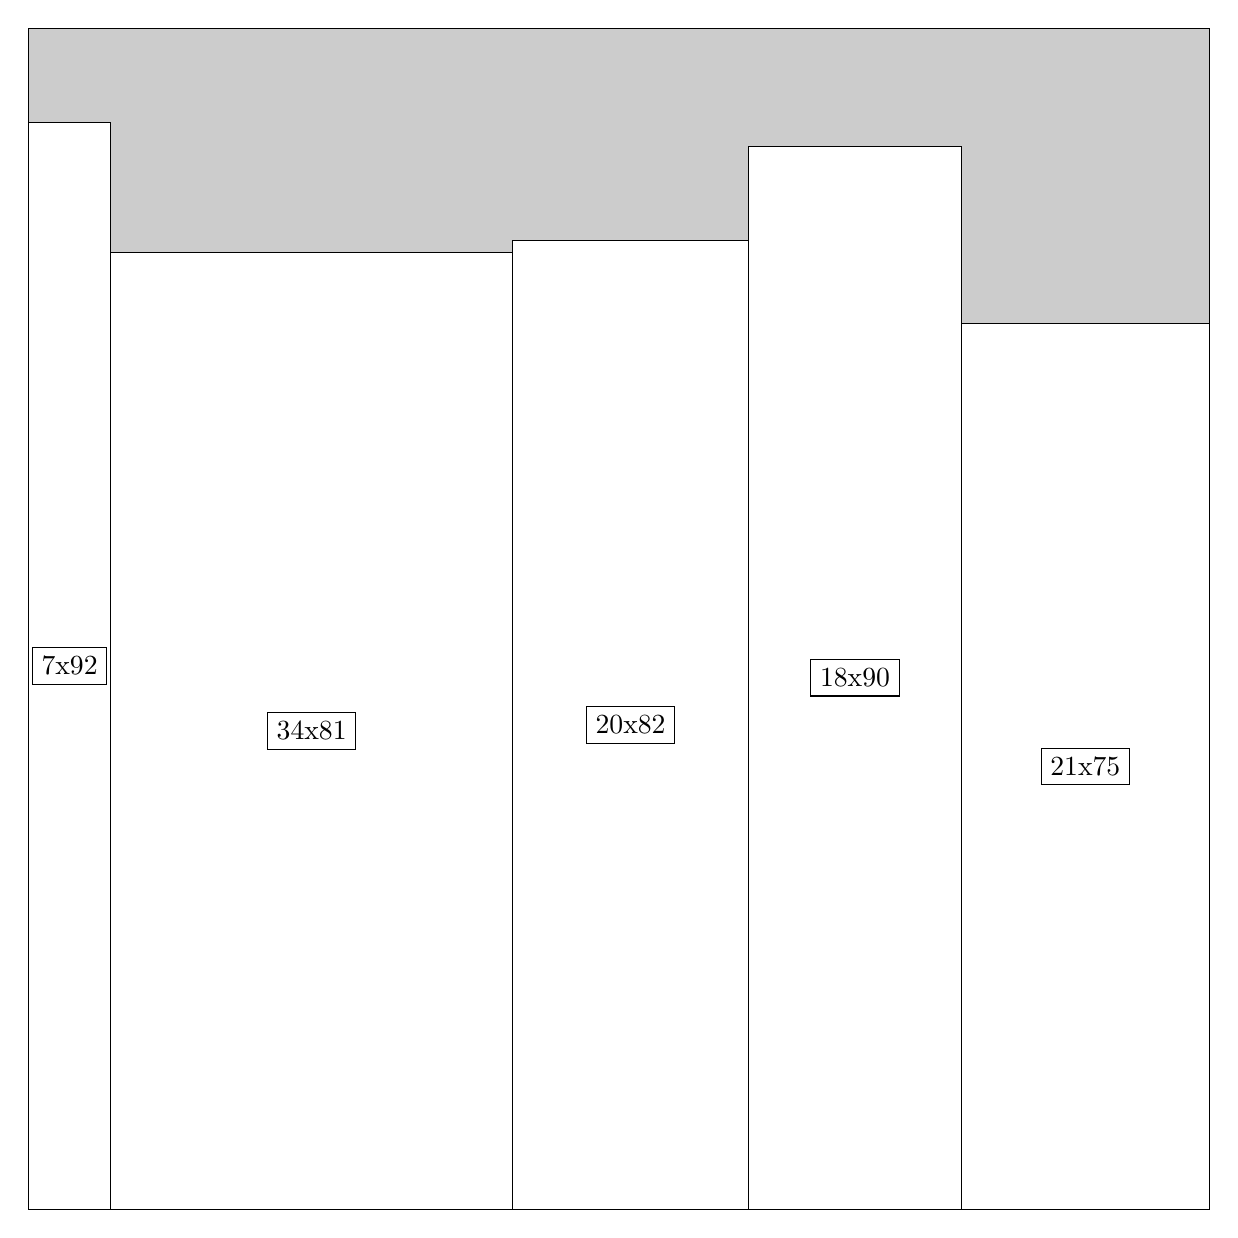
\begin{tikzpicture}[shorten >=1pt,scale=1.0,every node/.style={scale=1.0},->]
\tikzstyle{vertex}=[circle,fill=black!25,minimum size=14pt,inner sep=0pt]
\filldraw[fill=gray!40!white, draw=black] (0,0) rectangle (15.0,15.0);
\foreach \name/\x/\y/\w/\h in {7x92/0.0/0.0/1.05/13.799999999999999,34x81/1.05/0.0/5.1/12.15,20x82/6.1499999999999995/0.0/3.0/12.299999999999999,18x90/9.15/0.0/2.6999999999999997/13.5,21x75/11.85/0.0/3.15/11.25}
\filldraw[fill=white!40!white, draw=black] (\x,\y) rectangle node[draw] (\name) {\name} ++(\w,\h);
\end{tikzpicture}


w =7 , h =92 , x =0 , y =0 , v =644
\par
w =34 , h =81 , x =7 , y =0 , v =2754
\par
w =20 , h =82 , x =41 , y =0 , v =1640
\par
w =18 , h =90 , x =61 , y =0 , v =1620
\par
w =21 , h =75 , x =79 , y =0 , v =1575
\par
\newpage


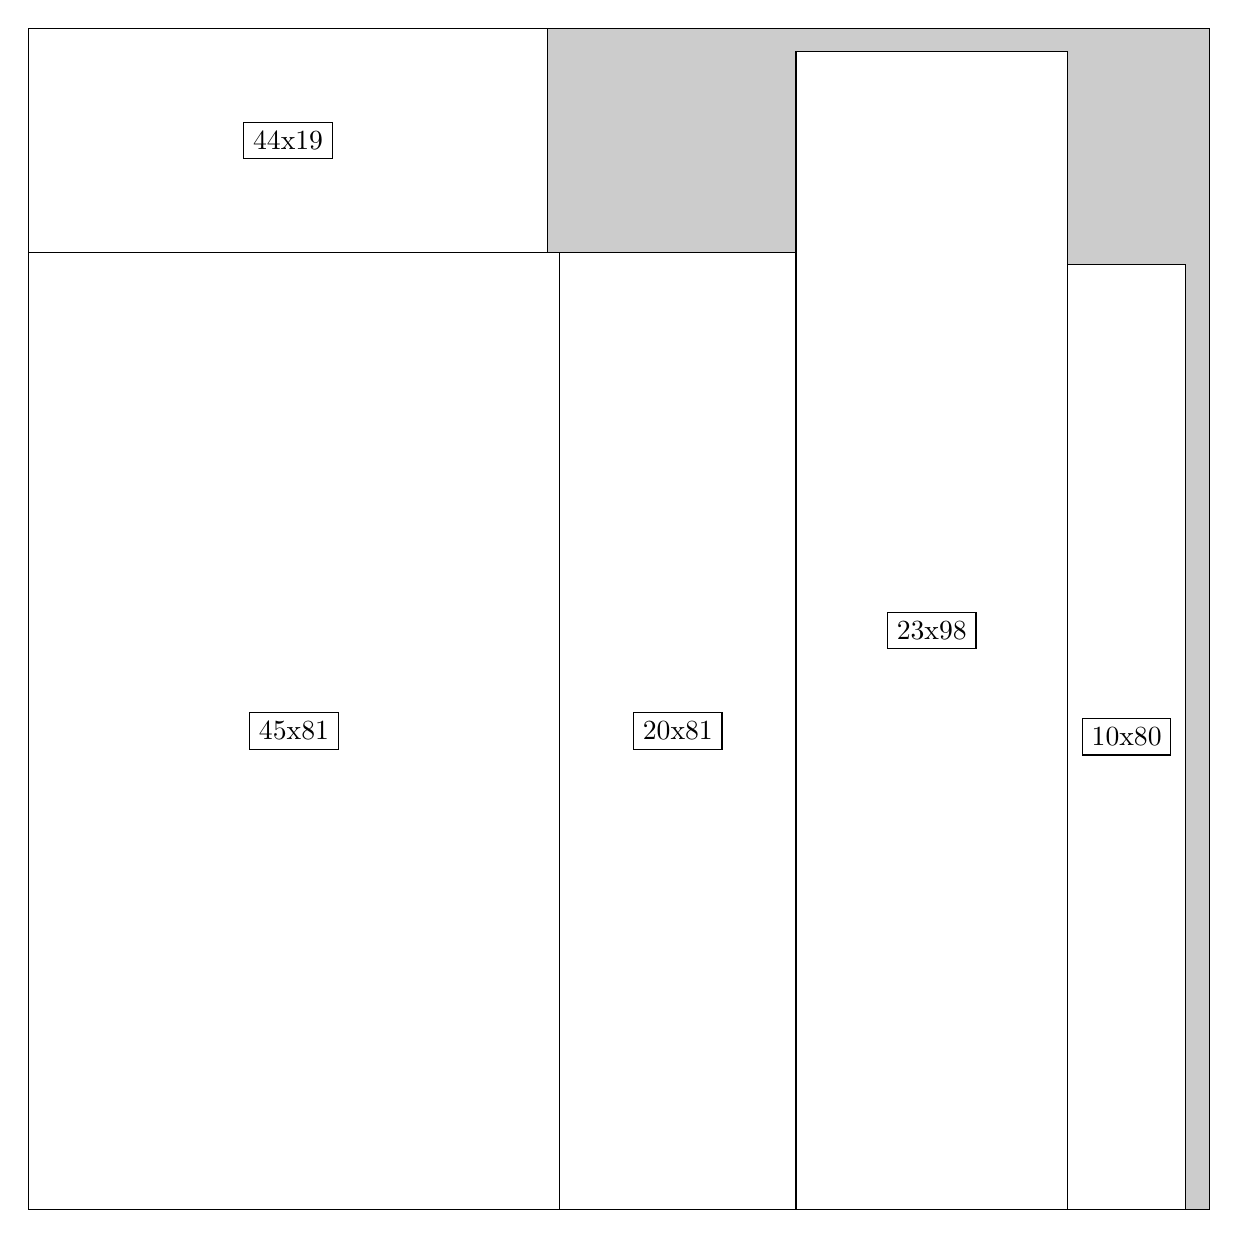
\begin{tikzpicture}[shorten >=1pt,scale=1.0,every node/.style={scale=1.0},->]
\tikzstyle{vertex}=[circle,fill=black!25,minimum size=14pt,inner sep=0pt]
\filldraw[fill=gray!40!white, draw=black] (0,0) rectangle (15.0,15.0);
\foreach \name/\x/\y/\w/\h in {45x81/0.0/0.0/6.75/12.15,23x98/9.75/0.0/3.4499999999999997/14.7,20x81/6.75/0.0/3.0/12.15,44x19/0.0/12.15/6.6/2.85,10x80/13.2/0.0/1.5/12.0}
\filldraw[fill=white!40!white, draw=black] (\x,\y) rectangle node[draw] (\name) {\name} ++(\w,\h);
\end{tikzpicture}


w =45 , h =81 , x =0 , y =0 , v =3645
\par
w =23 , h =98 , x =65 , y =0 , v =2254
\par
w =20 , h =81 , x =45 , y =0 , v =1620
\par
w =44 , h =19 , x =0 , y =81 , v =836
\par
w =10 , h =80 , x =88 , y =0 , v =800
\par
\newpage


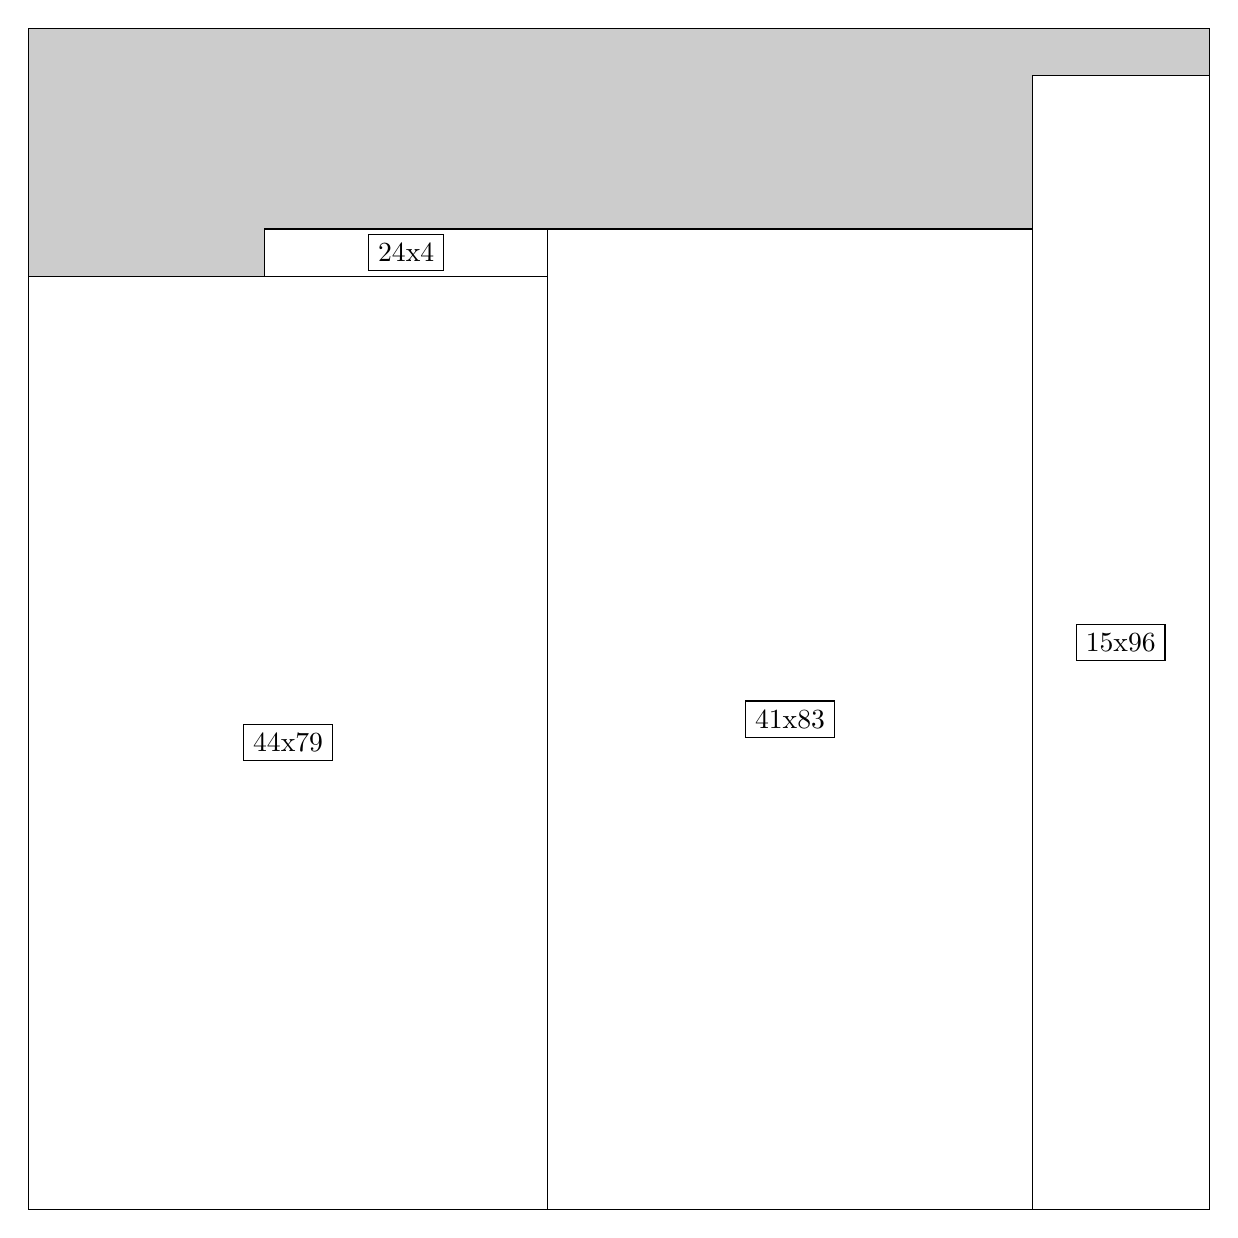
\begin{tikzpicture}[shorten >=1pt,scale=1.0,every node/.style={scale=1.0},->]
\tikzstyle{vertex}=[circle,fill=black!25,minimum size=14pt,inner sep=0pt]
\filldraw[fill=gray!40!white, draw=black] (0,0) rectangle (15.0,15.0);
\foreach \name/\x/\y/\w/\h in {44x79/0.0/0.0/6.6/11.85,41x83/6.6/0.0/6.1499999999999995/12.45,15x96/12.75/0.0/2.25/14.399999999999999,24x4/3.0/11.85/3.5999999999999996/0.6}
\filldraw[fill=white!40!white, draw=black] (\x,\y) rectangle node[draw] (\name) {\name} ++(\w,\h);
\end{tikzpicture}


w =44 , h =79 , x =0 , y =0 , v =3476
\par
w =41 , h =83 , x =44 , y =0 , v =3403
\par
w =15 , h =96 , x =85 , y =0 , v =1440
\par
w =24 , h =4 , x =20 , y =79 , v =96
\par
\newpage


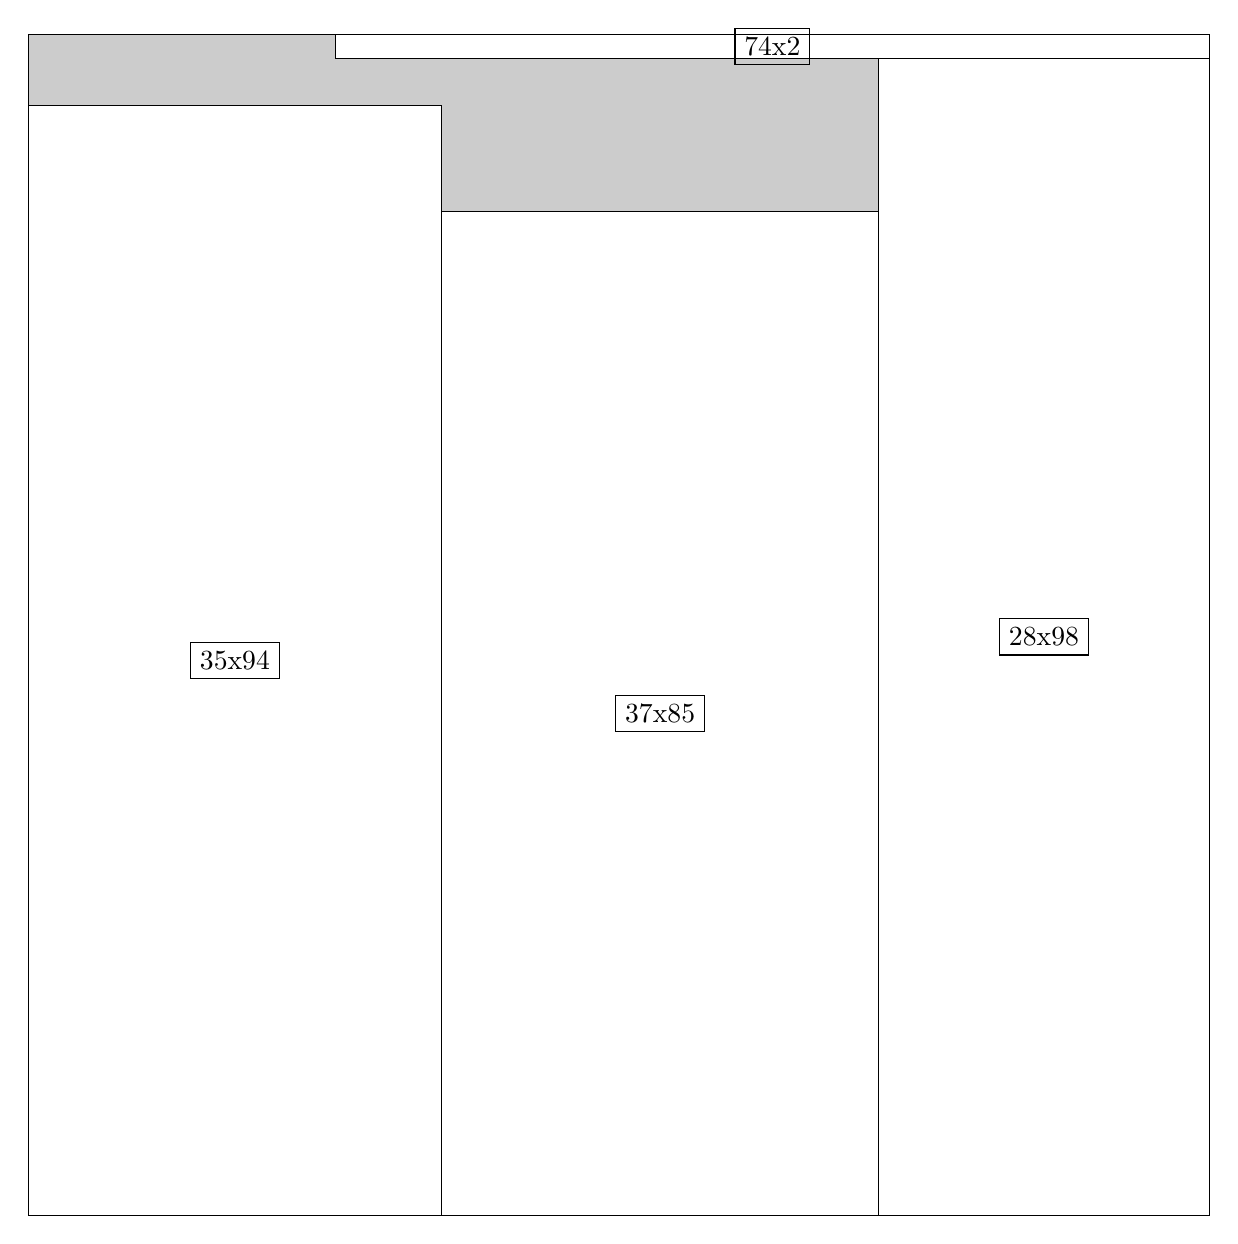
\begin{tikzpicture}[shorten >=1pt,scale=1.0,every node/.style={scale=1.0},->]
\tikzstyle{vertex}=[circle,fill=black!25,minimum size=14pt,inner sep=0pt]
\filldraw[fill=gray!40!white, draw=black] (0,0) rectangle (15.0,15.0);
\foreach \name/\x/\y/\w/\h in {35x94/0.0/0.0/5.25/14.1,37x85/5.25/0.0/5.55/12.75,28x98/10.799999999999999/0.0/4.2/14.7,74x2/3.9/14.7/11.1/0.3}
\filldraw[fill=white!40!white, draw=black] (\x,\y) rectangle node[draw] (\name) {\name} ++(\w,\h);
\end{tikzpicture}


w =35 , h =94 , x =0 , y =0 , v =3290
\par
w =37 , h =85 , x =35 , y =0 , v =3145
\par
w =28 , h =98 , x =72 , y =0 , v =2744
\par
w =74 , h =2 , x =26 , y =98 , v =148
\par
\newpage


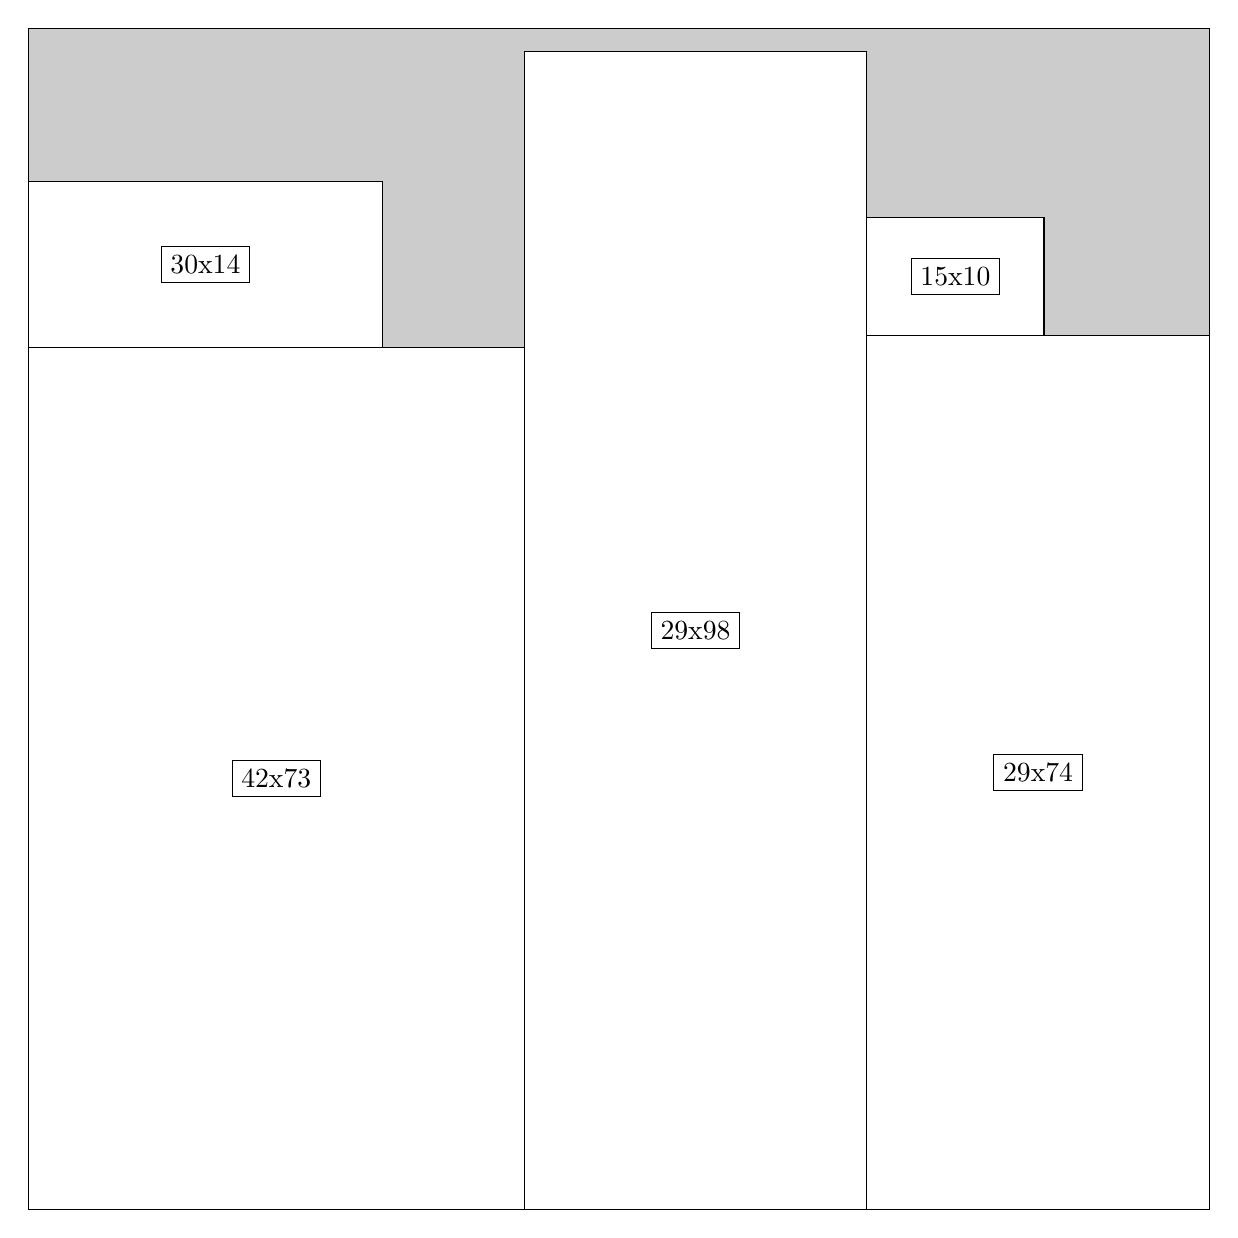
\begin{tikzpicture}[shorten >=1pt,scale=1.0,every node/.style={scale=1.0},->]
\tikzstyle{vertex}=[circle,fill=black!25,minimum size=14pt,inner sep=0pt]
\filldraw[fill=gray!40!white, draw=black] (0,0) rectangle (15.0,15.0);
\foreach \name/\x/\y/\w/\h in {42x73/0.0/0.0/6.3/10.95,29x98/6.3/0.0/4.35/14.7,29x74/10.65/0.0/4.35/11.1,30x14/0.0/10.95/4.5/2.1,15x10/10.65/11.1/2.25/1.5}
\filldraw[fill=white!40!white, draw=black] (\x,\y) rectangle node[draw] (\name) {\name} ++(\w,\h);
\end{tikzpicture}


w =42 , h =73 , x =0 , y =0 , v =3066
\par
w =29 , h =98 , x =42 , y =0 , v =2842
\par
w =29 , h =74 , x =71 , y =0 , v =2146
\par
w =30 , h =14 , x =0 , y =73 , v =420
\par
w =15 , h =10 , x =71 , y =74 , v =150
\par
\newpage


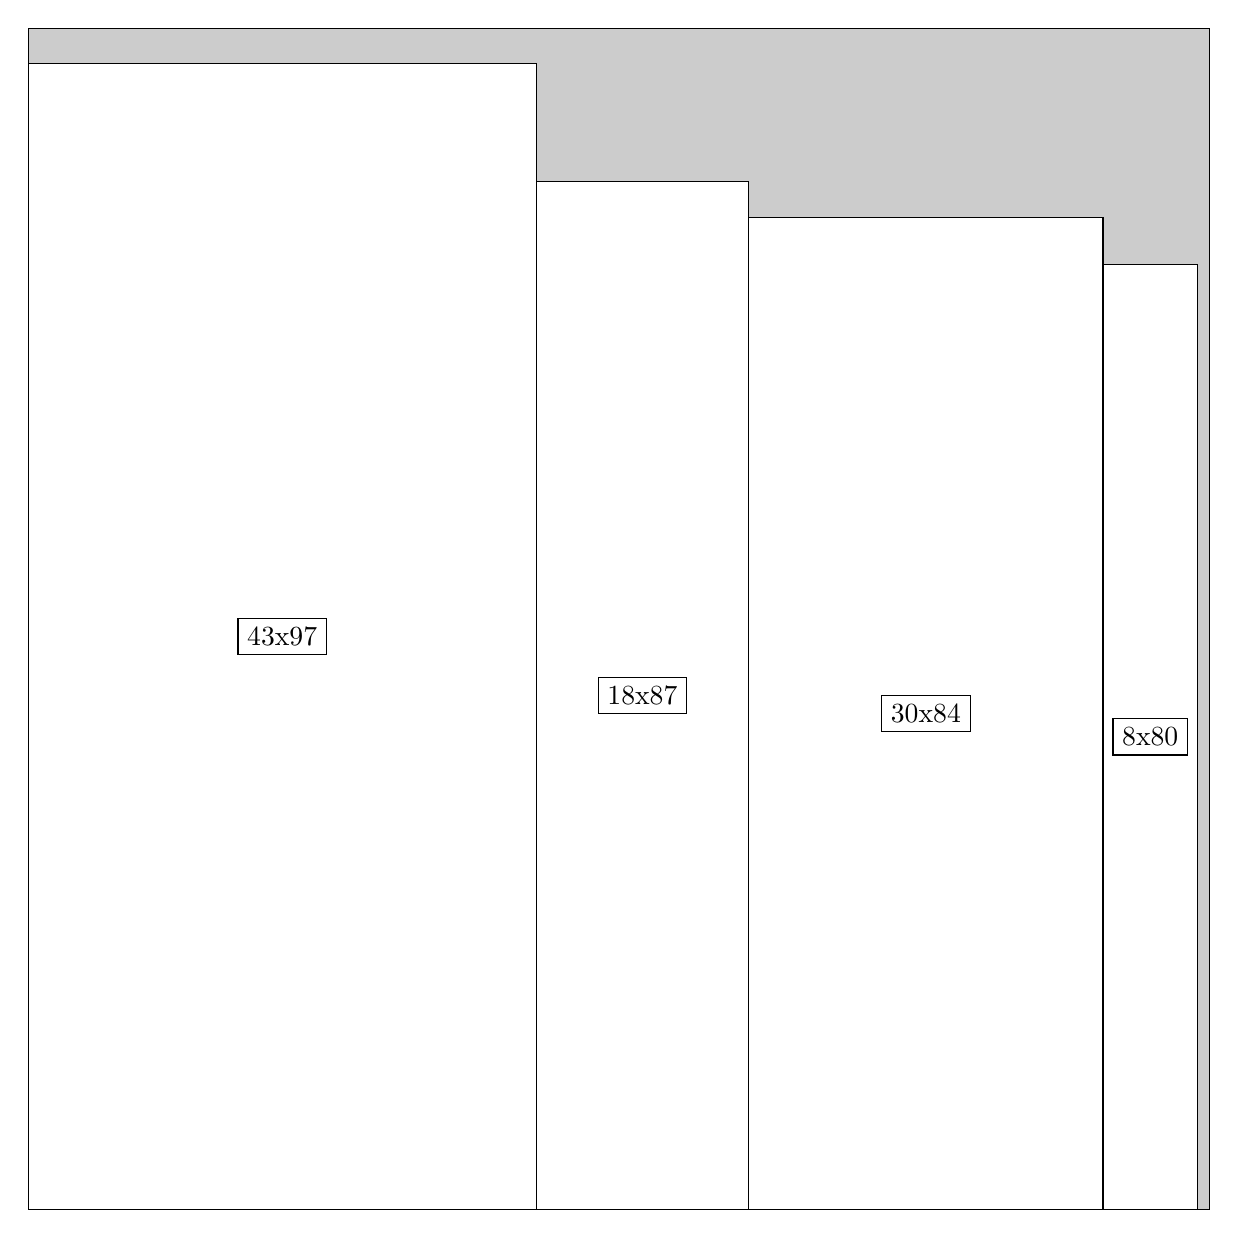
\begin{tikzpicture}[shorten >=1pt,scale=1.0,every node/.style={scale=1.0},->]
\tikzstyle{vertex}=[circle,fill=black!25,minimum size=14pt,inner sep=0pt]
\filldraw[fill=gray!40!white, draw=black] (0,0) rectangle (15.0,15.0);
\foreach \name/\x/\y/\w/\h in {43x97/0.0/0.0/6.45/14.549999999999999,30x84/9.15/0.0/4.5/12.6,18x87/6.45/0.0/2.6999999999999997/13.049999999999999,8x80/13.65/0.0/1.2/12.0}
\filldraw[fill=white!40!white, draw=black] (\x,\y) rectangle node[draw] (\name) {\name} ++(\w,\h);
\end{tikzpicture}


w =43 , h =97 , x =0 , y =0 , v =4171
\par
w =30 , h =84 , x =61 , y =0 , v =2520
\par
w =18 , h =87 , x =43 , y =0 , v =1566
\par
w =8 , h =80 , x =91 , y =0 , v =640
\par
\newpage


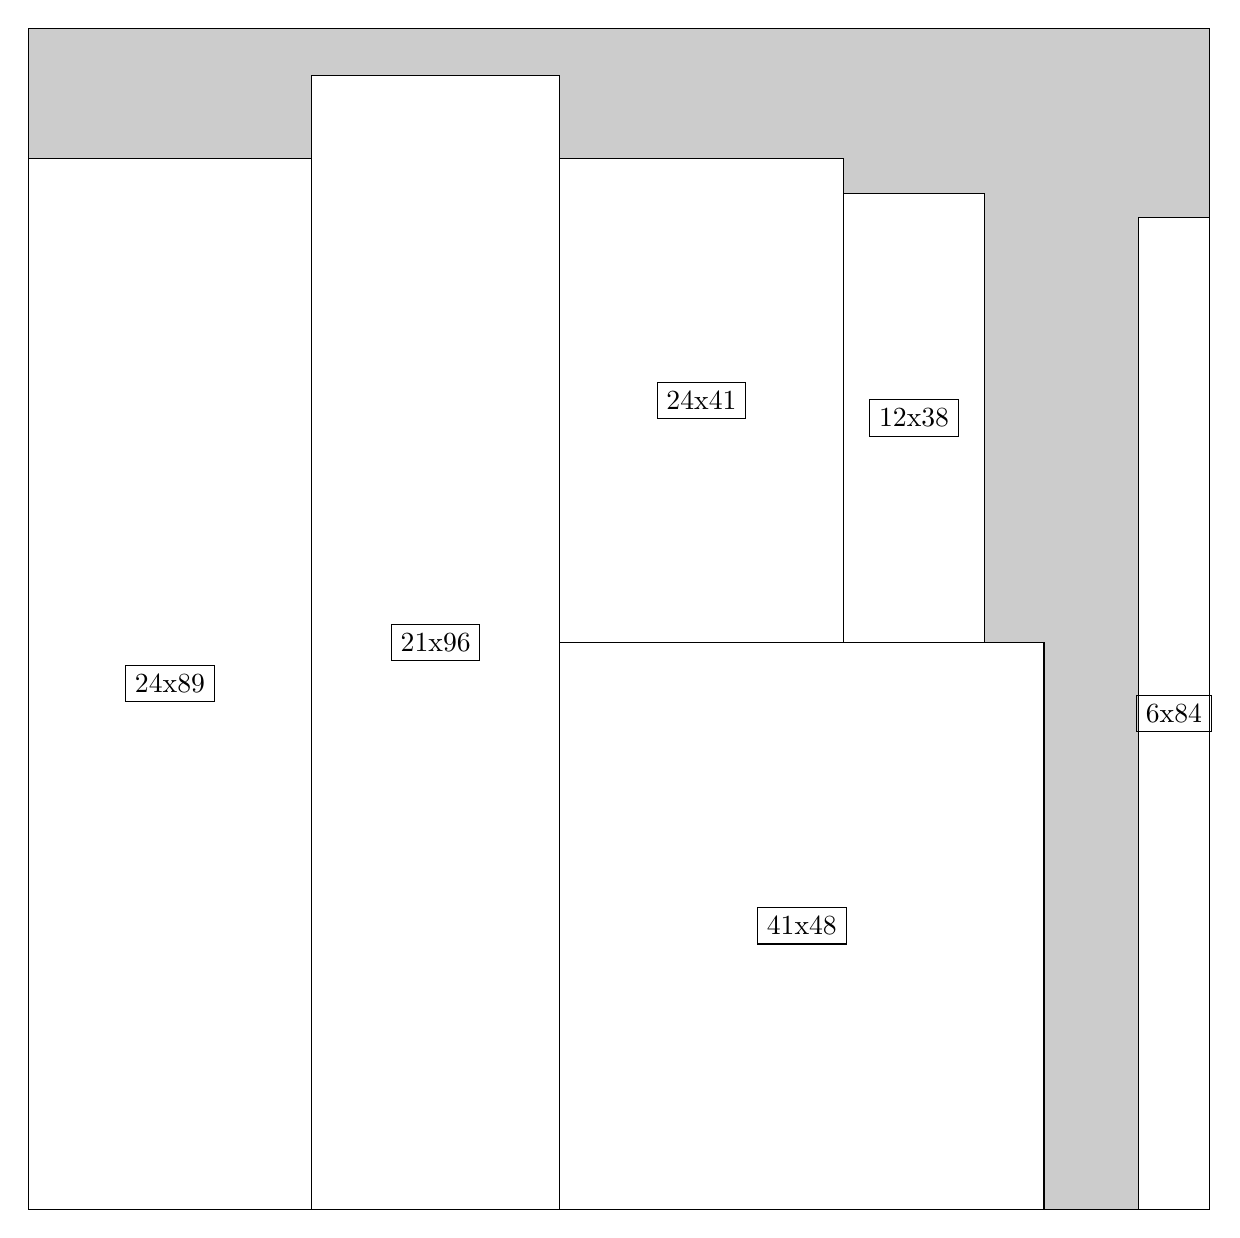
\begin{tikzpicture}[shorten >=1pt,scale=1.0,every node/.style={scale=1.0},->]
\tikzstyle{vertex}=[circle,fill=black!25,minimum size=14pt,inner sep=0pt]
\filldraw[fill=gray!40!white, draw=black] (0,0) rectangle (15.0,15.0);
\foreach \name/\x/\y/\w/\h in {24x89/0.0/0.0/3.5999999999999996/13.35,21x96/3.5999999999999996/0.0/3.15/14.399999999999999,41x48/6.75/0.0/6.1499999999999995/7.199999999999999,24x41/6.75/7.199999999999999/3.5999999999999996/6.1499999999999995,6x84/14.1/0.0/0.8999999999999999/12.6,12x38/10.35/7.199999999999999/1.7999999999999998/5.7}
\filldraw[fill=white!40!white, draw=black] (\x,\y) rectangle node[draw] (\name) {\name} ++(\w,\h);
\end{tikzpicture}


w =24 , h =89 , x =0 , y =0 , v =2136
\par
w =21 , h =96 , x =24 , y =0 , v =2016
\par
w =41 , h =48 , x =45 , y =0 , v =1968
\par
w =24 , h =41 , x =45 , y =48 , v =984
\par
w =6 , h =84 , x =94 , y =0 , v =504
\par
w =12 , h =38 , x =69 , y =48 , v =456
\par
\newpage


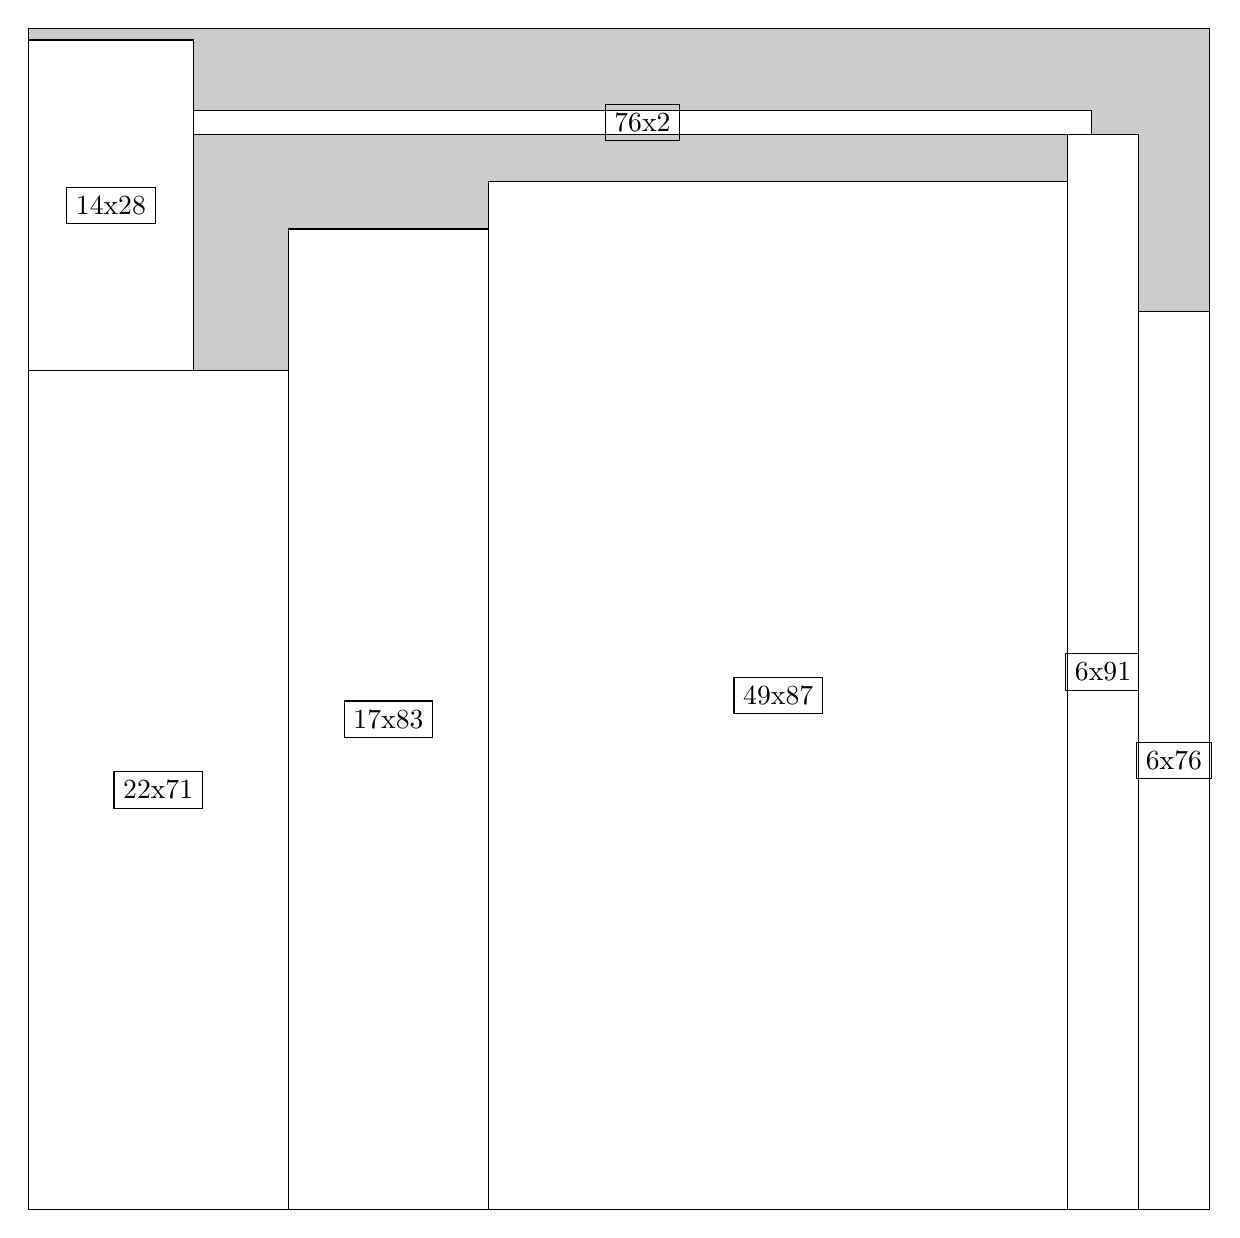
\begin{tikzpicture}[shorten >=1pt,scale=1.0,every node/.style={scale=1.0},->]
\tikzstyle{vertex}=[circle,fill=black!25,minimum size=14pt,inner sep=0pt]
\filldraw[fill=gray!40!white, draw=black] (0,0) rectangle (15.0,15.0);
\foreach \name/\x/\y/\w/\h in {22x71/0.0/0.0/3.3/10.65,17x83/3.3/0.0/2.55/12.45,49x87/5.85/0.0/7.35/13.049999999999999,6x91/13.2/0.0/0.8999999999999999/13.65,6x76/14.1/0.0/0.8999999999999999/11.4,14x28/0.0/10.65/2.1/4.2,76x2/2.1/13.65/11.4/0.3}
\filldraw[fill=white!40!white, draw=black] (\x,\y) rectangle node[draw] (\name) {\name} ++(\w,\h);
\end{tikzpicture}


w =22 , h =71 , x =0 , y =0 , v =1562
\par
w =17 , h =83 , x =22 , y =0 , v =1411
\par
w =49 , h =87 , x =39 , y =0 , v =4263
\par
w =6 , h =91 , x =88 , y =0 , v =546
\par
w =6 , h =76 , x =94 , y =0 , v =456
\par
w =14 , h =28 , x =0 , y =71 , v =392
\par
w =76 , h =2 , x =14 , y =91 , v =152
\par
\newpage


\end{document}